\documentclass[conference,letterpaper]{IEEEtran}
\IEEEoverridecommandlockouts
\usepackage{graphicx}
\usepackage{amsmath,amssymb}
\usepackage{booktabs}
\usepackage{array}
\usepackage{url}
\usepackage{balance}
\usepackage{microtype}
\usepackage[hidelinks]{hyperref}
\hypersetup{pdfauthor={Kasim Ishaque Ghanchi},pdftitle={Explanation Reliability and Failure Detection in Phishing URL Classification Under Dataset Shift},pdfsubject={CYCRAI 2027 research protocol}}
\setlength{\textfloatsep}{7pt}
\setlength{\floatsep}{5pt}
\setlength{\intextsep}{5pt}
\graphicspath{{figures/}}
\hyphenation{phish-ing over-fitting ex-plain-abil-ity}
\begin{document}
\title{Explanation Reliability and Failure Detection in Phishing URL Classification Under Dataset Shift}
\author{\IEEEauthorblockN{Kasim Ishaque Ghanchi}
\IEEEauthorblockA{Department of Computer Engineering\\
Mumbai, India\\
\href{mailto:kasimghanchi672@gmail.com}{kasimghanchi672@gmail.com}\\
\href{https://orcid.org/0009-0007-7444-9977}{ORCID: 0009-0007-7444-9977}}}
\maketitle
\begin{abstract}
High accuracy on a random test split does not establish that a phishing URL classifier will remain reliable on new domains or data collected through different pipelines. Nor does a plausible feature-attribution plot establish that its explanation is faithful to the classifier. This paper develops an auditable comparative protocol for evaluating prediction quality, explanation reliability, and the usefulness of explanations for identifying classification failures under dataset shift. It specifies matched lexical inputs; domain-disjoint and cross-corpus evaluation; logistic-regression and tree-ensemble baselines; SHAP and LIME explanation audits; and a held-out comparison of confidence-only, explanation-only, and combined error-warning rules. A descriptive comparison of two published datasets exposes a substantial class-prior difference: the published counts imply 62.9\% phishing URLs in LegitPhish and 10.4\% in URL-Phish. This difference motivates prior-aware evaluation and explicit checks for source artifacts. The resulting protocol identifies testable hypotheses, leakage controls, effect-size reporting, and a practical evidence standard for responsible deployment. This version reports verified literature-derived dataset statistics and a structured experimental plan; no new model-training or explanation-performance results are claimed.
\end{abstract}
\begin{IEEEkeywords}
explainable artificial intelligence, phishing URL detection, SHAP, LIME, domain shift, calibration, selective classification, responsible AI
\end{IEEEkeywords}

\section{Introduction}
Phishing URL classifiers often operate in an environment where suspicious domains, URL construction practices, and data acquisition processes change faster than model retraining cycles. An apparently strong benchmark result may therefore depend on accidental properties of how its dataset was assembled. Rashid \emph{et al.} documented impaired cross-dataset generalization in URL detection and showed that collection-related URL patterns can influence predictions \cite{rashid2024}. A later study identified duplication, inconsistent labels, and domain overrepresentation as additional threats to benchmarking \cite{datasetquality2025}. These problems affect not just the classifier, but also the interpretation of its decisions.

Explainable artificial intelligence (XAI) can expose influential URL features. LIME approximates a model locally through a simple surrogate \cite{ribeiro2016}; SHAP assigns additive feature contributions using a principled framework \cite{lundberg2017}. However, an explanation can be repeatable without being faithful, or intuitive without diagnosing when a model will fail. Randomization-based scrutiny has revealed limitations of visually convincing attribution methods in other domains \cite{adebayo2018}. Fidelity and sensitivity consequently warrant measurement instead of impressionistic inspection \cite{yeh2019}.

Recent phishing research already compares attribution techniques or examines temporal feature extraction \cite{panthi2026,mayo2026,limephish2025}. Merely drawing SHAP and LIME charts is thus not a sufficient contribution. The narrower question developed here is whether independently evaluated explanation-quality signals add useful information to confidence-based failure warnings on unseen domains and datasets.

The contributions of this \emph{research-protocol manuscript} are: (i) a leakage-aware comparison across group-disjoint and source-shift settings; (ii) an explicit audit of explanation faithfulness and reproducibility; (iii) a label-isolated evaluation of explanation-aware failure screening against strong uncertainty baselines; and (iv) a descriptive, independently verifiable audit of class balance in two recently published URL corpora. These are protocol and corpus-summary contributions, not experimental performance claims.

\section{Related Work and Research Gap}
\subsection{URL classification under shift}
A URL's length, punctuation, hostname structure, and character composition offer inexpensive signals for phishing detection. Dataset composition can nevertheless create shortcuts: for example, a crawler may collect benign HTTPS URLs more often than malicious HTTPS URLs. Rashid \emph{et al.} analyzed dataset-specific URL-prefix effects in cross-dataset experiments \cite{rashid2024}. Domain reuse and duplicate URLs further inflate randomly split scores, particularly when the same registered domain appears in train and test partitions \cite{datasetquality2025}.

\subsection{Feature attribution is not operational trust}
LIME and SHAP are complementary model-explanation tools \cite{ribeiro2016,lundberg2017}. Panthi \emph{et al.} compared these approaches for boosted phishing classifiers \cite{panthi2026}; Mayo \emph{et al.} investigated a temporally dynamic phishing feature pipeline with both methods \cite{mayo2026}. Another IEEE study assessed LIME across multiple classifiers using stability- and fidelity-related criteria \cite{limephish2025}. These works establish both the utility of local attribution and the risk of duplicating an explanation-only comparison.

\subsection{From probability to selective warnings}
Calibration evaluates whether probability estimates reflect observed frequencies; prediction confidence can be misleading even when top-label accuracy is high \cite{guo2017}. Selective classification allows a system to defer cases in exchange for lower error among the cases it does handle \cite{geifman2017}. The open empirical issue for this study is \emph{incremental value}: does adding explanation-quality information improve error detection or selective risk at matched coverage, after confidence and dataset shift are controlled?

\section{Research Questions and Hypotheses}
\textbf{RQ1:} How much do predictive quality and calibration change between ordinary random, registered-domain-disjoint, and cross-corpus tests? \textbf{H1:} Cross-corpus evaluation will generally be more challenging than a random in-source split, although the direction and magnitude must be measured.

\textbf{RQ2:} Do SHAP and LIME explanations remain faithful and reproducible when the evaluation population changes? \textbf{H2:} Their rankings and perturbation responses may differ across model families and test sources; the protocol does not presuppose a winner.

\textbf{RQ3:} Can explanation-derived evidence identify misclassified URLs better than confidence alone? \textbf{H3:} A combined rule may add information, but its incremental benefit must be demonstrated with paired uncertainty intervals and held-out tests.

\textbf{RQ4:} Are models exploiting dataset-source artifacts rather than phishing-relevant structure? \textbf{H4:} Predictable source identity from lexical features, or sharp feature-prevalence differences, would signal a confounding risk rather than prove causal shortcut use.

\section{Datasets and Published Corpus Audit}
Two independently published corpora are candidate evaluation sources. Potpelwar \emph{et al.} describe LegitPhish, with reported phishing and legitimate counts of 63,678 and 37,540 \cite{legitphish2025}. Linh and Hung describe URL-Phish, comprising 11,660 phishing and 100,000 benign URLs \cite{urlphish2025}. Table~\ref{tab:datasets} uses the \emph{class counts reported by the authors}; Fig.~\ref{fig:balance} visualizes their proportions. These values are not outcomes of our experiments.

\begin{table}[!t]
\caption{Published URL Corpus Counts (Not Study Measurements)}\label{tab:datasets}
\centering\footnotesize
\begin{tabular}{lrrr}
\toprule
Dataset & Phishing & Benign & Phishing share\\
\midrule
LegitPhish \cite{legitphish2025} & 63,678 & 37,540 & 62.9\%\\
URL-Phish \cite{urlphish2025} & 11,660 & 100,000 & 10.4\%\\
\bottomrule
\end{tabular}
\end{table}

\begin{figure}[!t]
\centering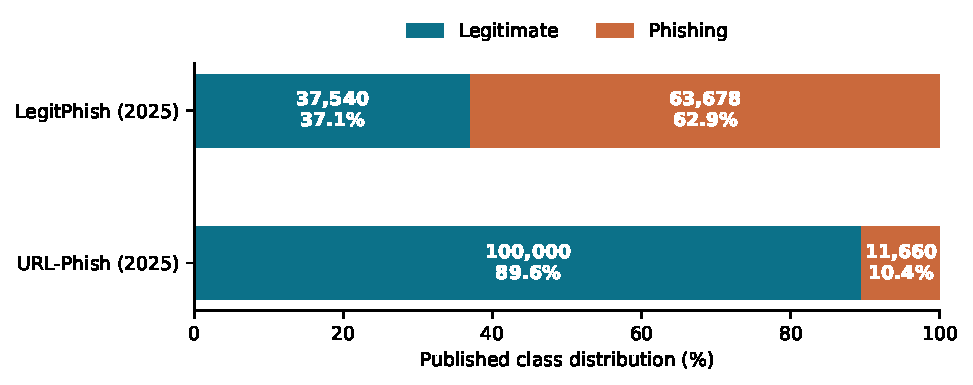
\includegraphics[width=\columnwidth]{published_dataset_balance.pdf}
\caption{Class composition calculated from published class counts \cite{legitphish2025,urlphish2025}; no classifiers were trained to generate this plot.}\label{fig:balance}
\end{figure}

A numerical inconsistency requires disclosure: the two LegitPhish class counts sum to 101,218, whereas its published text also reports a total of 101,219 \cite{legitphish2025}. The plot and table therefore use the component counts and neither silently repair nor explain away the one-record discrepancy. Raw-file verification is mandatory before modeling. Label encodings also differ: LegitPhish reports phishing as 0, while URL-Phish reports phishing as 1. Both must be normalized to a unified target \(y=1\) for phishing. Cross-corpus comparisons should share a freshly recomputed feature extractor rather than rely on differently implemented supplied columns.

\section{Proposed Experimental Design}
\subsection{Data integrity and splits}
After obtaining the files from their cited repositories, retain raw URL strings and original labels, log version and checksum, strip exact duplicate URLs, and flag contradictory labels. Canonicalization should be conservative because rewriting URL paths or queries can alter real behavior. Normalize scheme and host case for grouping only, preserving the original URL for feature extraction. Use a maintained public-suffix list to derive registered-domain groups; discard malformed examples under a recorded rule. Partition training, tuning, and in-source testing by \emph{registered domain}, then test on the independent corpus after removing train/test domain collisions. When collection timestamps are trustworthy, add a forward-time experiment; do not imply a temporal test merely because papers were published in different years.

\begin{figure*}[!t]
\centering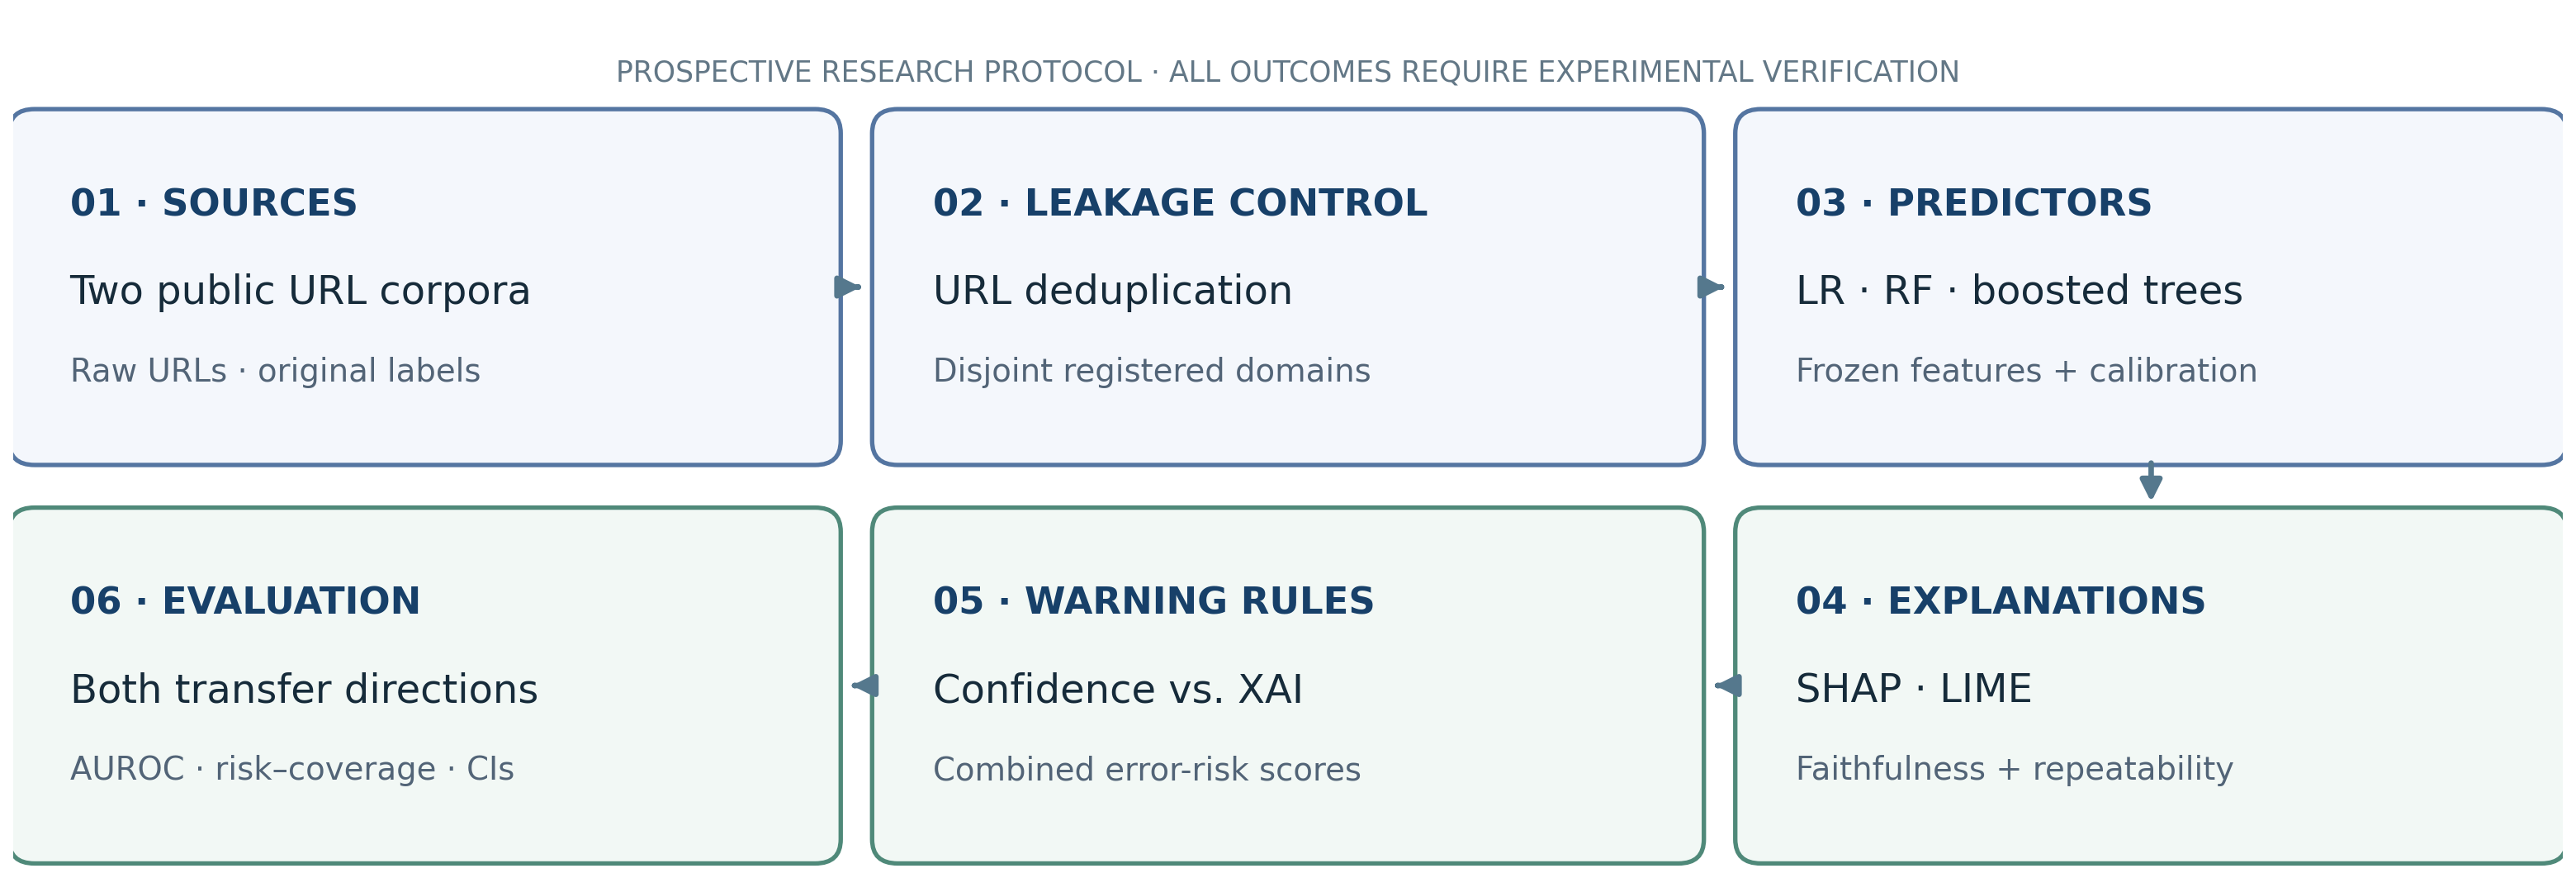
\includegraphics[width=.96\textwidth]{research_workflow.png}
\caption{Proposed research workflow: datasets, data-leakage prevention, classifiers, explanation audits, warning rules, and cross-corpus evaluation. This is a design diagram, not a measured result.}\label{fig:pipeline}
\end{figure*}

\subsection{Features, models, and controls}
Compute the same lexical and structural features from both corpora: URL and hostname lengths; counts of dots, digits, hyphens, separators, and special symbols; query length; URL character entropy; subdomain count; IP-literal indicator; and explicit HTTPS scheme indicator. Avoid WHOIS age, live page content, reputation lookups, and blacklist membership in the primary benchmark because they require source-dependent acquisition at prediction time and can silently leak labels. Include three transparent-to-complex baselines: standardized logistic regression, random forest, and gradient-boosted trees. Tune on group-disjoint validation data with a fixed budget and publish the search space, seeds, and hardware.

\subsection{Explanations and faithfulness checks}
Use model-appropriate SHAP implementations and model-agnostic LIME under clearly recorded backgrounds, random seeds, perturbation budgets, and explanation sample counts. Compare top-\(k\) feature overlap and rank correlation when both methods are defined on the same feature representation. A deletion test replaces the top-ranked features with training-distribution reference values and measures prediction change, contrasted against matched random-feature deletion. Because independently replacing correlated lexical features can create implausible vectors, this is a \emph{model-probe proxy}, not evidence of real-world causal importance. Report both fidelity and explanation-runtime distributions, including failure cases.

For observation \(x\), classifier \(f\), attribution vector \(a(x)\), and masked feature set \(M_k(x)\) selected from the top-\(k\) attributions, define a normalized deletion response
\begin{equation}
D_k(x)=|f(x)-f(T_{M_k}(x))|,
\end{equation}
where \(T\) is a declared reference-value transform. Report \(\Delta D_k=D_k-D_k^{\mathrm{random}}\) with paired uncertainty intervals rather than treating a large unadjusted drop as proof of explanation validity. Explanation-repeatability can be estimated by average top-\(k\) Jaccard agreement across independent LIME runs, while deterministic SHAP should be stress-tested with alternative admissible background samples.

\subsection{Error-warning ablation}
Define \(e_i=\mathbb{1}[\hat y_i\neq y_i]\). On \emph{validation data only}, fit a low-capacity warning model predicting \(e_i\) using: A) confidence/entropy; B) attribution-stability and deletion-response measures; and C) their combination. Compare each against a confidence-only baseline on strictly untouched test examples. Attribution features must depend only on \(x_i\), trained model outputs, and declared reference data: evaluation labels must never enter feature computation. Calibration is fitted on a held-out tuning partition and frozen prior to cross-corpus evaluation. The central estimand is
\begin{equation}
\Delta_{\mathrm{AUROC}}=\mathrm{AUROC}(s_C,e)-\mathrm{AUROC}(s_A,e),
\end{equation}
where \(s_C\) denotes combined error-risk score and \(s_A\) confidence-only risk. A positive point estimate is not persuasive without an uncertainty interval and testing across both transfer directions.

\begin{figure}[!t]
\centering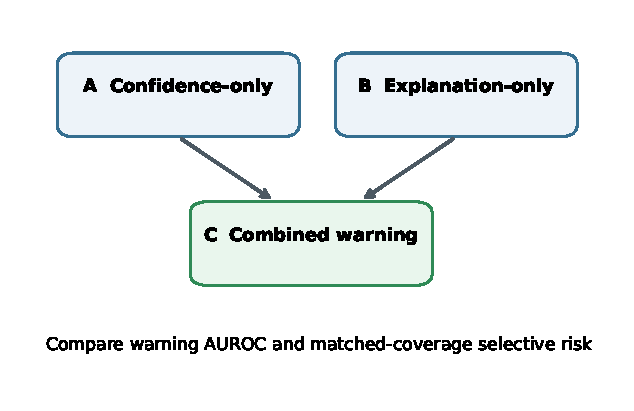
\includegraphics[width=\columnwidth]{ablation_schema.pdf}
\caption{Planned, not measured, comparison of confidence-only, explanation-only, and combined warnings.}\label{fig:ablation}
\end{figure}

\subsection{Reporting metrics and statistical analysis}
For classification, report phishing precision/recall/F1, average precision, AUROC, false-positive rate, and confusion matrices under both raw and clearly specified class-prior-adjusted test populations. For probability quality, report Brier score and reliability diagrams; calibration within the training domain does not ensure calibration after shift \cite{guo2017}. For safety-relevant deferral, sort by warning score and report risk \(R(c)\) among the retained fraction \(c\), with matched-coverage differences and area under the risk-coverage curve \cite{geifman2017}. For explanation quality, report deletion-minus-random response, seed stability, top-\(k\) agreement, and per-example runtime.

Replicate domain splits across at least five predefined seeds, retaining domain grouping in resampling. Calculate bootstrap 95\% intervals by resampling \emph{registered-domain clusters}, not individual near-duplicate URLs. Show effect sizes and paired differences; avoid using uncorrected multiple significance tests as the principal evidence. Ablate URL components that could betray source collection (e.g., HTTPS prevalence) and fit a source-identity classifier on the common lexical features as a diagnostic. A strong source discriminator alone is not proof that the phishing model used a specific spurious shortcut.


\section{Study Status and Reporting Boundaries}
The present document is a reproducible \emph{comparative study design} supported by a literature-derived corpus audit. It deliberately contains no newly measured F1 scores, AUROC gains, stability coefficients, SHAP importance rankings, or risk-coverage outcomes. Producing any such value without downloading the datasets, executing the split and model pipelines, and retaining logs would be fabrication. The attached executable starter pipeline creates actual performance plots only when supplied with licensed source files and explicitly specified label encodings.

Table~\ref{tab:matrix} states the evidence required for a defensible subsequent results version. A valid negative result---for instance, no benefit from explanations beyond calibrated confidence---would be scientifically informative and should be reported rather than suppressed. The main novelty, if empirically supported, would be evidence about \emph{incremental explanation utility under shift}, not invention of SHAP, LIME, or a generic phishing classifier.

\begin{table}[!t]
\caption{Planned Comparisons (Measurements Pending)}\label{tab:matrix}
\centering\footnotesize\setlength{\tabcolsep}{3pt}
\begin{tabular}{@{}p{.31\columnwidth}p{.62\columnwidth}@{}}
\toprule
Comparison & Target metric and control\\
\midrule
Random / group split & F1, AUROC; no registered-domain overlap\\
Within / cross-source & F1, Brier; identical lexical extraction\\
SHAP / LIME & Deletion contrast, rank stability; matched cases\\
Confidence / combined & Error AUROC, selective risk; held-out labels\\
URL artifact ablation & Transfer gap; logged feature removal\\
\bottomrule
\end{tabular}
\end{table}

\section{Threats to Validity and Responsible Use}
\textbf{Selection and label bias.} Both candidate datasets depend on particular benign and malicious collection practices; transfer scores mix differences in class prevalence, collection time, and source pipelines. Neither corpus alone establishes deployment prevalence. Contradictory labels and duplicated domains must be quantified.

\textbf{Explanation perturbation artifacts.} Feature deletion can leave the manifold of valid URLs, and SHAP explanations depend on the choice of background and feature dependence assumptions. Stability is not causality, and explanation agreement need not mean correctness. Human comprehensibility would require a separate reader study.

\textbf{Security and privacy.} Examples are analyzed as \emph{strings}; the benchmark must not visit suspicious URLs or resolve malicious hosts. The shared reproducibility package should avoid posting active harmful links in rendered figures, remove personal data accidentally embedded in URLs, and preserve source attribution. Results can support analyst triage but should not be presented as an autonomous safety guarantee.

\textbf{Evaluation honesty.} A paper becomes an empirical conference submission only when experiments and validation are complete. Working code, environment versions, dataset checksums, excluded records, exact split groups, random seeds, and plots should accompany any numerical claims. Sponsorship or acceptance decisions are outside the scope of research results.

\section{Conclusion}
Responsible phishing detection requires more than accurate predictions and attractive attribution graphics. This paper specifies a testable comparison that separates model performance, explanation faithfulness, and confidence-conditioned failure screening, and it makes domain and dataset shift first-class evaluation settings. Published counts from two candidate datasets already reveal materially different phishing prevalences, underscoring the need for careful priors and source-leakage checks. Whether explanations genuinely improve detection of model errors remains an empirical question. Answering it with leakage-safe data splits, measured explanation fidelity, paired confidence baselines, and reproducible evidence is the next step toward a defensible CYCRAI submission.

\begin{thebibliography}{99}
\bibitem{ribeiro2016} M. T. Ribeiro, S. Singh, and C. Guestrin, ``Why should I trust you?: Explaining the predictions of any classifier,'' in \emph{Proc. ACM SIGKDD}, 2016, pp. 1135--1144, doi: 10.1145/2939672.2939778.
\bibitem{lundberg2017} S. M. Lundberg and S.-I. Lee, ``A unified approach to interpreting model predictions,'' in \emph{Advances in Neural Information Processing Systems}, vol. 30, 2017, pp. 4765--4774.
\bibitem{adebayo2018} J. Adebayo \emph{et al.}, ``Sanity checks for saliency maps,'' in \emph{Advances in Neural Information Processing Systems}, vol. 31, 2018.
\bibitem{yeh2019} C.-K. Yeh, C.-Y. Hsieh, A. S. Suggala, D. I. Inouye, and P. K. Ravikumar, ``On the (in)fidelity and sensitivity of explanations,'' in \emph{Advances in Neural Information Processing Systems}, vol. 32, 2019.
\bibitem{rashid2024} F. Rashid, B. Doyle, S. C. Han, and S. Seneviratne, ``Phishing URL detection generalisation using unsupervised domain adaptation,'' \emph{Computer Networks}, vol. 245, 2024, Art. no. 110398, doi: 10.1016/j.comnet.2024.110398.
\bibitem{datasetquality2025} P. Afonso, E. Maia, I. Amorim, and I. Praça, ``Rethinking phishing detection: How dataset quality affects model generalization,'' in \emph{Proc. 15th Int. Conf. Advanced Computer Information Technologies}, 2025, pp. 542--547, doi: 10.1109/ACIT65614.2025.11185656.
\bibitem{legitphish2025} R. S. Potpelwar, U. V. Kulkarni, and J. M. Waghmare, ``LegitPhish: A large-scale annotated dataset for URL-based phishing detection,'' \emph{Data in Brief}, vol. 63, 2025, Art. no. 111972, doi: 10.1016/j.dib.2025.111972.
\bibitem{urlphish2025} D. M. Linh and T. C. Hung, ``A feature-engineered dataset of benign and phishing URLs for machine learning and large language models evaluation,'' \emph{Data in Brief}, vol. 63, 2025, Art. no. 112162, doi: 10.1016/j.dib.2025.112162.
\bibitem{guo2017} C. Guo, G. Pleiss, Y. Sun, and K. Q. Weinberger, ``On calibration of modern neural networks,'' in \emph{Proc. 34th Int. Conf. Machine Learning}, 2017, pp. 1321--1330.
\bibitem{geifman2017} Y. Geifman and R. El-Yaniv, ``Selective classification for deep neural networks,'' in \emph{Advances in Neural Information Processing Systems}, vol. 30, 2017, pp. 4878--4887.
\bibitem{panthi2026} S. Panthi, M. Patidar, K. Zalawadia, D. Vekariya, and V. Vekariya, ``A performance analysis of SHAP and LIME for interpreting boosting models in phishing URL detection,'' \emph{Scientific Reports}, Aug. 2026, doi: 10.1038/s41598-026-66800-x.
\bibitem{mayo2026} C. Mayo, M. Tchuindjang, S. Brohi, and N. Ersotelos, ``A temporally dynamic feature-extraction framework for phishing detection with LIME and SHAP explanations,'' \emph{Future Internet}, vol. 18, no. 2, Art. no. 101, 2026, doi: 10.3390/fi18020101.
\bibitem{limephish2025} D. A. Fatih, A. Hamonangan, and T. Hidayat, ``Evaluating LIME-based explainability for phishing URL detection across multiple machine learning models,'' in \emph{Proc. IEEE Int. Conf. Emerging Trends in Information Systems and Informatics}, Dec. 2025, doi: 10.1109/ICETISI67983.2025.11406019.
\end{thebibliography}
\end{document}
